\documentclass[10pt,journal,compsoc]{IEEEtran}

\usepackage[utf8]{inputenc}
\usepackage{amsmath,amssymb,amsfonts}
\usepackage{graphicx}
\usepackage{booktabs}
\usepackage{hyperref}
\usepackage{subcaption}
\usepackage{microtype}
\usepackage{cite}

\hypersetup{
    colorlinks=true,
    linkcolor=blue,
    citecolor=cyan,
    urlcolor=blue
}

\begin{document}

\title{Normalizing Flows and Unpaired Image-to-Image Translation with CycleGAN\\
\large Assignment 2 -- Deep Generative Models (Fall 1404 / 2025)}

\author{Alireza Najafi Motiei (Student ID: 810100224)\\
\IEEEmembership{Faculty of Electrical and Computer Engineering, University of Tehran}\\
Instructor: Dr. Mostafa Tavassolipour}

\markboth{University of Tehran, ECE Department -- Deep Generative Models (Fall 1404)}{Najafi Motiei: Assignment 2 Report}

\maketitle

\begin{abstract}
This report documents Assignment 2 of Deep Generative Models (Fall 1404). In the first section, we examine Normalizing Flows (NFs), focusing on the Masked Autoencoder for Distribution Estimation (MADE) and the Masked Autoregressive Flow (MAF) architecture. We analyze the duality between MAF and Inverse Autoregressive Flow (IAF) regarding training versus sampling parallelism, and demonstrate unsupervised anomaly detection using exact log-likelihoods, achieving $\text{AUROC} = 0.73$. In the second section, we explore Cycle-Consistent Adversarial Networks (CycleGAN) for unpaired image-to-image translation. We analyze the theoretical necessity of the cycle-consistency and identity mapping objectives, contrast U-Net and ResNet generator architectures, study the 70$\times$70 PatchGAN discriminator with historical image buffers, and evaluate empirical performance on the Horse2Zebra and Apple2Orange benchmarks.
\end{abstract}

\begin{IEEEkeywords}
Normalizing Flows, MADE, MAF, IAF, Anomaly Detection, AUROC, CycleGAN, Pix2Pix, PatchGAN, Unpaired Image Translation, Horse2Zebra, Apple2Orange.
\end{IEEEkeywords}

\section{Question 1: Normalizing Flows}

\subsection{Architectural Formulation: MADE and MAF}
Normalizing flows transform a simple base distribution $p_Z(z)$ (typically $\mathcal{N}(0, I)$) into a complex empirical distribution $p_X(x)$ via a sequence of invertible and differentiable mappings $f: \mathcal{Z} \to \mathcal{X}$. By the change-of-variables theorem:
\begin{equation}
\log p_X(x) = \log p_Z(f^{-1}(x)) + \log \left| \det \left( \frac{\partial f^{-1}(x)}{\partial x} \right) \right|
\end{equation}

\subsubsection{Masked Autoencoder for Distribution Estimation (MADE)}
MADE enforces the autoregressive property—$p(x) = \prod_{i=1}^D p(x_i \mid x_{<i})$—in feedforward networks via binary masking of weight matrices. Each hidden neuron is assigned an integer degree $m(l)$, ensuring that neuron $j$ in layer $l$ only connects to neurons in layer $l-1$ with degrees $m(l-1) \le m(l)$.

\subsubsection{Masked Autoregressive Flow (MAF)}
MAF leverages MADE to parameterize affine scale and translation functions:
\begin{equation}
x_i = z_i \exp(\alpha_i(x_{<i})) + \mu_i(x_{<i}) \iff z_i = (x_i - \mu_i) \exp(-\alpha_i)
\end{equation}
Due to the triangular structure of $\frac{\partial z}{\partial x}$, the log-determinant of the Jacobian simplifies to a sum over scale terms:
\begin{equation}
\log \left| \det J \right| = -\sum_{i=1}^D \alpha_i
\end{equation}
In our implementation, seven stacked MADE blocks were employed to balance representational capacity with computational tractability.

\begin{figure}[htbp]
\centering

\includegraphics[width=0.9\columnwidth]{figures/image10.png}
\caption{MAF training convergence and negative log-likelihood curve.}
\label{fig:maf_loss}
\end{figure}

\subsection{Sampling Duality: MAF versus IAF}
During training, MAF evaluates all $x_i$ simultaneously, enabling full parallelization across dimensions. However, sequential generation $x_i \sim p(x_i \mid x_{<i})$ requires $D$ serial forward passes. In our experiments, training required $756.81$ seconds, whereas synthesizing five images sequentially took $1995.75$ seconds.

Conversely, Inverse Autoregressive Flow (IAF) defines:
\begin{equation}
x_i = z_i \exp(\alpha_i(z_{<i})) + \mu_i(z_{<i})
\end{equation}
Since all $z \sim \mathcal{N}(0, I)$ are drawn concurrently, IAF generates full samples in a single forward pass, but suffers from serial evaluation during training.

\begin{figure}[htbp]
\centering

\includegraphics[width=0.85\columnwidth]{figures/image13.png}
\caption{Synthesized samples generated via sequential inversion from MAF.}
\label{fig:maf_samples}
\end{figure}

\subsection{Unsupervised Anomaly Detection}
Traditional accuracy metrics are unsuitable for anomaly detection due to extreme class imbalance ($95\%$ normal vs. $5\%$ anomalous). We assess performance using:
\begin{enumerate}
    \item \textbf{AUROC}: Threshold-independent discriminative performance.
    \item \textbf{AUPR}: Precision-recall dynamics focusing on the anomalous class.
    \item \textbf{Optimal F1-Score}: Best achievable harmonic balance.
\end{enumerate}

\begin{figure}[htbp]
\centering

\includegraphics[width=0.85\columnwidth]{figures/image5.png}
\caption{Anomaly detection ROC and Precision-Recall curves yielding an $\text{AUROC} = 0.73$.}
\label{fig:roc}
\end{figure}

Using the negative log-likelihood $-\log p(x)$ as the anomaly score, the model maps anomalous samples to low-density regions, achieving an $\text{AUROC} = 0.73$. Importantly, reconstructing anomalies via $x \to z \to \hat{x}$ in an NF cannot detect anomalies because bidirectional bijectivity guarantees near-zero reconstruction error across all inputs.

\section{Question 2: Cycle-Consistent Adversarial Networks (CycleGAN)}

\subsection{Theoretical Framework}
In the absence of paired training examples $(x_i, y_i)$, learning mappings $G: X \to Y$ and $F: Y \to X$ is severely under-constrained.

\subsubsection{Total Objective Formulation}
The complete CycleGAN objective comprises:
\begin{equation}
\mathcal{L}(G, F, D_X, D_Y) = \mathcal{L}_{\text{GAN}}(G, D_Y) + \mathcal{L}_{\text{GAN}}(F, D_X) + \lambda_{\text{cyc}} \mathcal{L}_{\text{cyc}} + \lambda_{\text{id}} \mathcal{L}_{\text{id}}
\end{equation}
where the cycle-consistency loss is defined as:
\begin{equation}
\mathcal{L}_{\text{cyc}}(G, F) = \mathbb{E}_{x \sim p_{\text{data}}(x)} [\|F(G(x)) - x\|_1] + \mathbb{E}_{y \sim p_{\text{data}}(y)} [\|G(F(y)) - y\|_1]
\end{equation}
Without $\mathcal{L}_{\text{cyc}}$, the generators are susceptible to mode collapse, mapping arbitrary inputs to a singular realistic sample in the target domain.

\subsubsection{Identity Mapping Regularizer}
The identity loss $\mathcal{L}_{\text{id}}(G, F) = \mathbb{E}_y [\|G(y) - y\|_1] + \mathbb{E}_x [\|F(x) - x\|_1]$ encourages the generator to act as an identity operator when presented with target-domain samples. This prevents unnecessary color and tonal shifts in non-target regions (e.g., background vegetation).

\subsection{Architectural Considerations}
\begin{itemize}
    \item \textbf{U-Net vs. ResNet}: Pix2Pix employs U-Net with skip connections to preserve exact pixel alignment. CycleGAN utilizes a ResNet backbone with downsampling, residual bottleneck blocks, and upsampling. The bottleneck forces the model to encode abstract semantic representations and alter textures without being constrained by rigid low-level spatial skip connections.
    \item \textbf{70$\times$70 PatchGAN}: Discriminators classify $70 \times 70$ overlapping image patches rather than outputting a single global scalar, capturing high-frequency local textures while conserving parameters.
    \item \textbf{Replay Image Buffer}: A historical buffer storing the 50 most recently generated images stabilizes discriminator training, dampening oscillations between alternating generator modes.
\end{itemize}

\subsection{Experimental Results}

\subsubsection{Horse2Zebra Benchmark ($\lambda_{\text{id}} = 0$)}
Trained on $128 \times 128$ crops with $\lambda_{\text{cyc}} = 10$. The generator successfully synthesizes realistic zebra stripe patterns on horses. However, in the absence of identity regularization, the background grass and sky undergo minor tinting.

\begin{figure}[htbp]
\centering
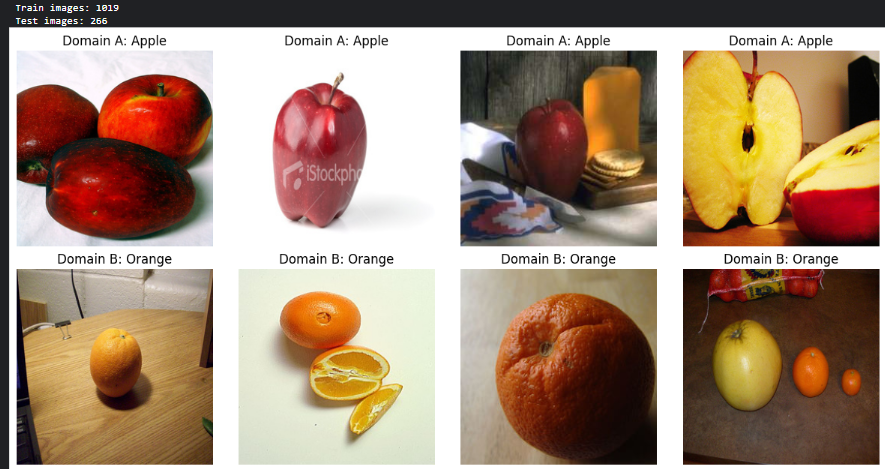
\includegraphics[width=0.95\columnwidth]{figures/image25.png}
\caption{CycleGAN translations on Horse2Zebra: Original inputs (left), generated zebra/horse mappings (middle), and cyclic reconstructions (right).}
\label{fig:h2z}
\end{figure}

\begin{figure}[htbp]
\centering
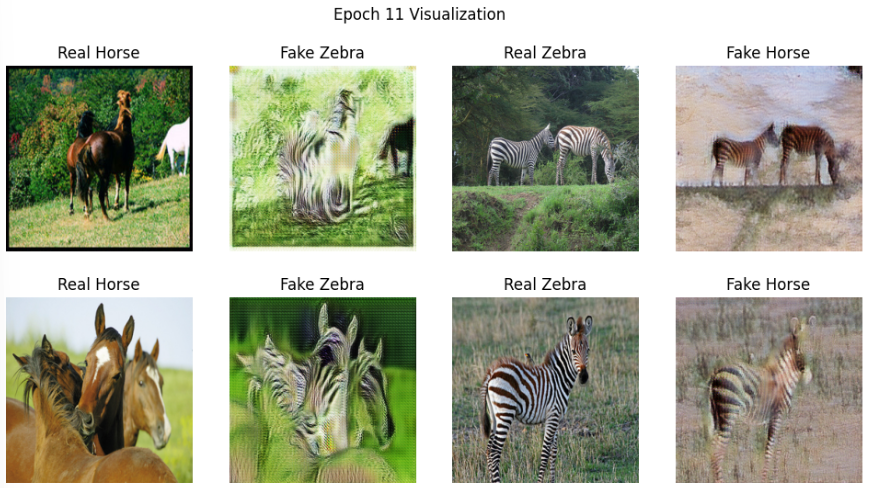
\includegraphics[width=0.95\columnwidth]{figures/image21.png}
\caption{Training loss trajectories on Horse2Zebra across generator, discriminator, and cycle-consistency objectives.}
\label{fig:cyclegan_loss}
\end{figure}

\subsubsection{Apple2Orange Benchmark ($\lambda_{\text{id}} = 5$)}
Incorporating $\lambda_{\text{id}} = 5$ dramatically preserves background scene neutrality. The model modifies the color palette and surface texture of apples into oranges while maintaining unchanged surrounding surfaces.

\begin{figure}[htbp]
\centering
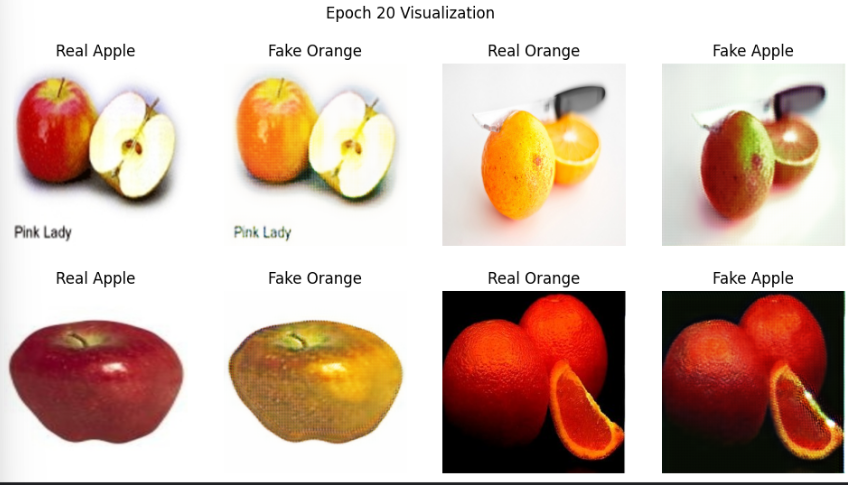
\includegraphics[width=0.95\columnwidth]{figures/image35.png}
\caption{CycleGAN translations on Apple2Orange illustrating texture modification while preserving background color composition via identity regularization.}
\label{fig:a2o}
\end{figure}

\bibliographystyle{IEEEtran}
\begin{thebibliography}{1}
\bibitem{germain2015made}
M.~Germain, K.~Gregor, I.~Murray, and H.~Larochelle, ``MADE: Masked autoencoder for distribution estimation,'' in \emph{ICML}, 2015.
\bibitem{papamakarios2017masked}
G.~Papamakarios, T.~Pavlakou, and I.~Murray, ``Masked autoregressive flow for density estimation,'' in \emph{NeurIPS}, 2017.
\bibitem{zhu2017unpaired}
J.-Y. Zhu, T.~Park, P.~Isola, and A.~A. Efros, ``Unpaired image-to-image translation using cycle-consistent adversarial networks,'' in \emph{IEEE ICCV}, 2017.
\bibitem{isola2017image}
P.~Isola, J.-Y. Zhu, T.~Zhou, and A.~A. Efros, ``Image-to-image translation with conditional adversarial networks,'' in \emph{IEEE CVPR}, 2017.
\end{thebibliography}

\end{document}
